\section{Charm in the Cloud}
\label{sec:cloud}

% {\color{blue}
% Points to cover
% \begin{itemize} 
%     \item Q. How to solve scaling issues in the cloud?
%     \item Avoid wasted computations
%         \begin{itemize}
%             \item Short circuit
%             \item Leverage locality of gateways (only use a subset of gateways  or decoding)
%         \end{itemize}
%     \item Spatial partitioning helps correctness and performance
%         \begin{itemize}
%             \item Leverage locality
%             \item Leverage timing
%         \end{itemize}
%     \item Shorter transmissions help scalability
% \end{itemize}
% }

At the cloud, \name\ seeks to coherently combine received signals from multiple gateways to recover weak received signals. At a high level, \name\ collates I/Q samples from multiple gateways and estimates their packet start time and wireless channel. It then uses standard coherent SIMO combining (see Sec.~\ref{sec:simo}) of the same weak transmission across multiple gateways to ensure that the data can be accurately recovered. \name\ repeats this cloud-based PHY-layer processing at city scale across clients and gateways. 

The rest of this section describes the key challenges and opportunities in making the above design scalable and practical. First, we describe \name's approach to ensure accurate time-synchronization between gateways -- showing how even an offset of one or two samples can be severely detrimental to coherent combining. Second, we present our solution to dynamically infer signals from which gateways need to be combined over time to best recover a weak signal. Finally, we present opportunities to improve bandwidth and system performance at the cloud by avoiding wasted transmissions of I/Q data to the cloud as well as wasted computation.



\subsection{Time Synchronization at the Cloud}
\name\ relies on the accurate timing of received weak signals at the gateways for two important reasons: First, any offset in timing between signals corresponding to the same packet across  gateways will prevent the signals from coherently combining. Second, the precise start time of packets across gateways is valuable information to identify the packet, allowing \name\ to infer which received signals across gateways correspond to the same packet.

A naive approach to synchronize base stations would be to synchronize them through highly accurate clocks (GPS-synced) or through time-synchronization protocols in software over the backbone network (e.g. NTP). In practice, for indoor gateways (e.g. set top boxes) connected to an Ethernet backhaul, these can provide time synchronization of up to a few milliseconds. In practical terms, this means that the received signals at the gateways can be time synchronized to within a small number of time samples. 

\begin{figure}
    \centering
    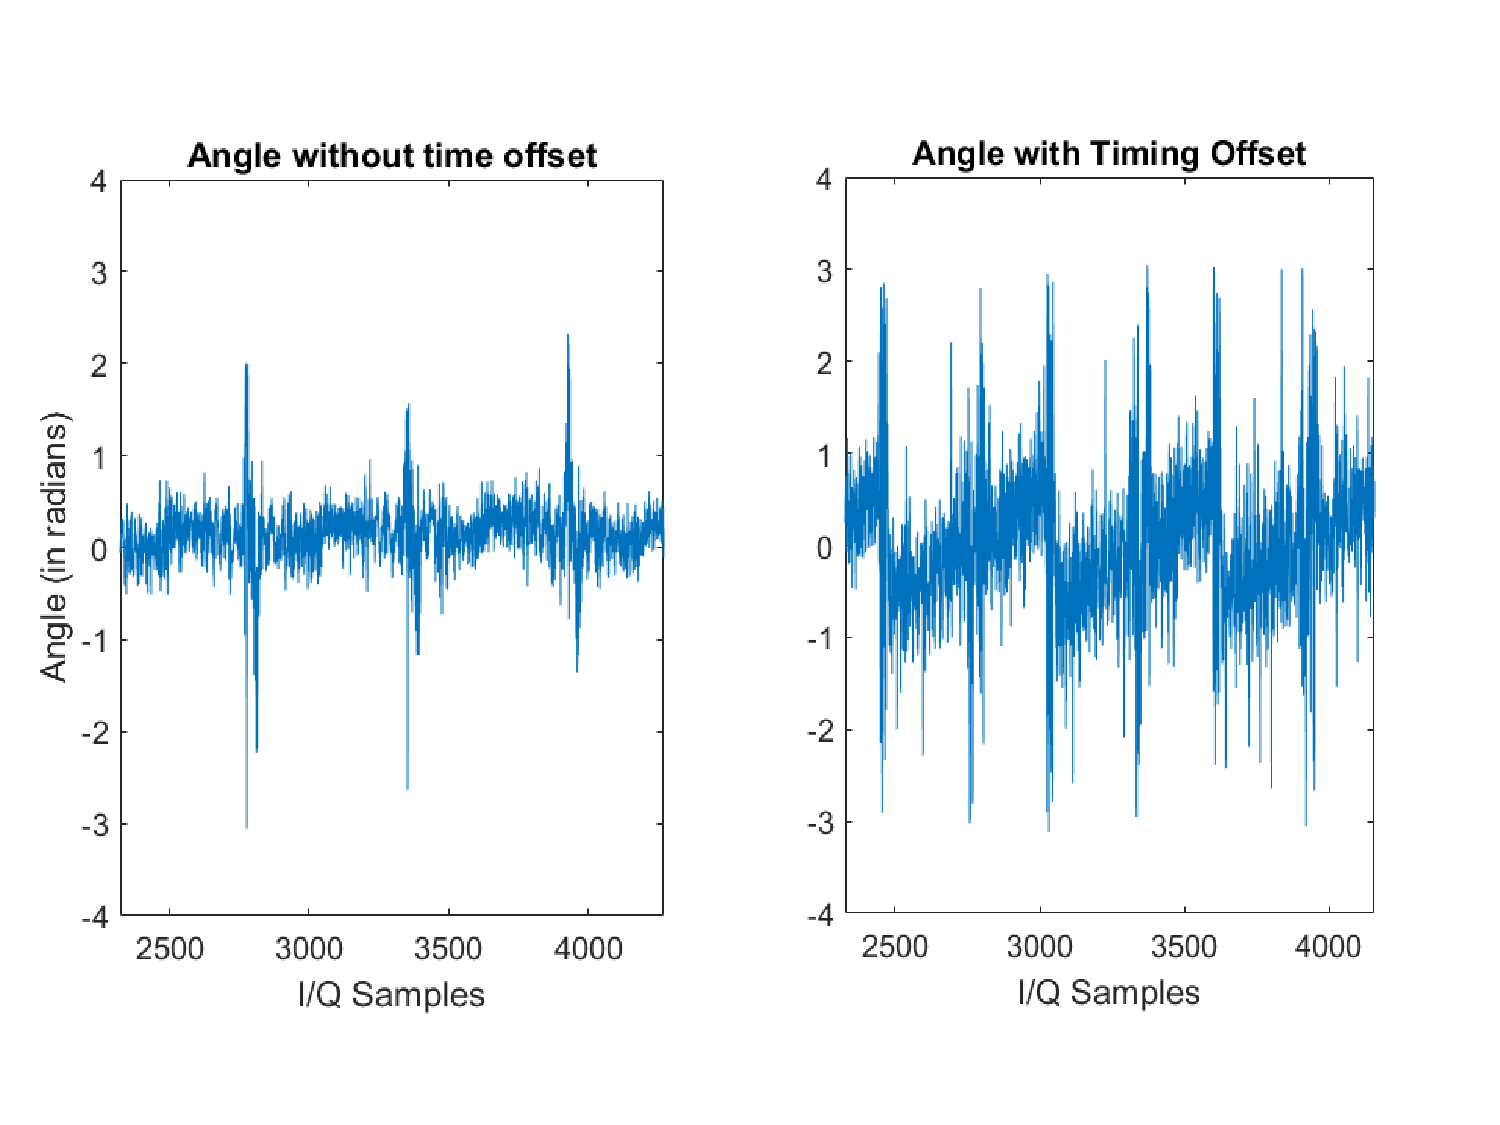
\includegraphics[width=0.45\textwidth, height=1.6in]{figures/TimeOffset.pdf}
    \vspace*{-0.1in}
    \caption{Effect of timing offset on detection}
        \vspace*{-0.0in}

    \label{fig:toffset}
    \compactimg
\end{figure}

Unfortunately, even a small offset in the timing between two gateways can severely deteriorate coherent combining. Fig.~\ref{fig:toffset} depicts a simple example of the phase difference between two gateways whose signals are offset by zero and one sample respectively. We note that even an offset of one frequency bin causes a significant time-varying error in phase between the gateways. As a result, summing up these signals would cause some symbols in-phase to reinforce, while others that are out-of-phase cancel each other. \vspace*{0.1in}

\noindent {\bf Phase-Based Time-Sync Below the Noise: } \name\ overcomes this challenge by recognizing that small time-errors between two gateways results in a phase difference over time that is predictable. As shown in Fig.~\ref{fig:toffset}, this phase difference is a linear function of time, given by $2\pi f(t) \delta t$, where $f(t)$ is the instantaneous frequency of the chirp (linear in time) and $\delta t$ is the required timing offset. In principle, one can therefore estimate the slope in phase over time to recover the timing offset. In practice however, doing so is challenging, particularly when each received signal at each gateway is completely buried below the noise. The phase of such signals at any such gateway simply appears to be random -- making any form of linear regression of the slope highly error-prone.

\name\ overcomes this challenge using two key properties: First, owing to coarse time synchronization of the gateways (via NTP), any residual timing error between them is limited to a few samples. This allows \name\ to iteratively optimize over a small number of time-shifts to infer the offset that leads to the best fit. Second, \name's can extract timing offsets both from the preamble and the data symbols. To see how, notice that our approach only considers the {\it difference} in phase between the same packet heard at two different gateways. Given that, in the absence of timing offsets, both gateways perceive the same underlying message bits over time, the resulting phase difference would be independent of the transmitted data bits -- whether they belong to the preamble or data. 

\name's approach therefore considers a the range of possible small offsets between any two received signal sequences. For each candidate offset, it computes the phase difference between the signals as a function of time. It then identifies the true offset between the gateways as the one whose phase difference varies minimally across the entire packet. Given that our approach averages measurements through the entire packet (both preamble and data), it remains highly resilient to noise.\vspace*{0.1in}


\noindent {\bf Maintaining Synchronization across Packets: } Finally, \name\ can learn the time-offsets between gateways, particularly in busy urban deployments, by using information from past packets. Recall that \name's coherent is only affected by timing errors between pairs of gateways -- not the gateway and any particular client. While these errors may change over time, over small intervals (e.g. hundreds of milliseconds), they are unlikely to change. As a result, one can use the measured time offset from a previous packet to infer the offset at the next packet that follows soon after. This allows us to maintain a history of the time-offsets, smoothed by algorithms such as Kalman filtering with outlier rejection, that helps us better predict time offsets between gateways even when signals from certain clients are too weak to measure these reliably. 



% What are the big challenges at the cloud? Why is it hard?

% Biggest issue is scalability with many gateways. Larger problem due to user deployed gateways.

% Another issue: latency. But LoRaWAN is not as sensitive to it.

% Why is it hard?

% Too many streams, and every stream may not have 

\subsection{Joint Decoding at the Cloud}
\label{sec:joint-decoding-cloud}
This section answers an important question: How does \name\ decide which weak signals received from a set of gateways need to be combined coherently? In other words, \name\ must identify which signals at the gateway correspond to the same packet from the same transmitter. It must do so even in the presence of overlapping transmissions from multiple clients at geographically different locations. \vspace*{0.1in}

\noindent {\bf Who should we combine?: } \name\ addresses this challenge by using the timing information of packets to infer transmissions that correspond to the same user. It further uses the perceived signal-to-noise ratios and geographic location of the gateways and measures the likelihood that far-away gateways can listen to transmissions from the users at the observed signal-to-noise ratios. It then calculates a feature vector for each received signal that contains two tuple: (1) The time instance at which the packet was received; and (2) The geographic location of the gateway. We apply the OPTICS clustering algorithm~\cite{ankerst1999optics} to then cluster received signals from multiple clients at any time instance. 

Past-clustering, we combine received signals from a subset of clients in each cluster. Specifically, we only choose to combine signals with a sufficiently high signal-to-noise ratio. This is because transmissions that are highly noisy tend to add little additional value yet cost uplink bandwidth. 

An important consequence of our clustering approach based on geographic location of the gateway is that it facilitates spatial re-use. Specifically, it is quite possible that weak transmissions from two different neighborhoods occur at the same time but are heard at distinct subsets of gateways. \name\ allows us to decode these transmissions simultaneously without mixing up their signals. Indeed, gateways that are geographically in-between and hear interfering signals from both clients can be simply weeded out from clustering due to their poor signal-to-noise ratio. 

 \vspace*{0.1in}

\noindent {\bf Joint Decoding Algorithm: } Algorithm~\ref{alg:algorithm-label} below describes \name's joint-decoding algorithm end-to-end. At a high level, our approach retrieves the wireless channels of the signals to be combined at any instance, their timing offsets and frequency offsets computed as described in the above sections. We, then eliminate any phase errors owing to time and frequency offsets in the received signals. We then coherently sum up the resulting signals multiplied by the conjugate channels as described in Sec.~\ref{sec:background}. 



%{\color{red} Swarun: (Add if room) Joint decoding pseudo-code to summarize the story with MIMO math}

\RestyleAlgo{boxruled}
\LinesNumbered
\begin{algorithm}[ht]
\caption{Joint decoding algorithm}
\label{alg:algorithm-label}
 packets = receive\_data(candidates)\;
 \For{p in packets}{
 p = $e^{j2\pi (\Delta_f)t}$ p \tcp*{Freq Offset Correction}
 p = $e^{j2\pi f(\Delta_t)}$ p \tcp*{Timing Offset Correction}
 h(p)$=\frac{p}{reference}$ \tcp*{Channel Estimation}
 }
 combined\_packet$=$zeros(p)\;
 \For{p in packets}{
 combined\_packet = combined\_packet + h$^*$p \;
 }
 decode(combined\_packet)\;
 SEND ACK\;
 
 \end{algorithm}

% In this section, we describe how \name\ decides signals from which packets need to be combined over time to be decoded 

% The objective of this protocol is to enable scaleable joint decoding of LoRa
% transmissions given internet bandwidth limitations between the gateways and
% and the cloud-based decoder.

% {\color{blue} High-level algorithm description:
% \begin{itemize}
%     \item Sent detection information
%     \item Cloud server clusters potential receptions
%     \item Request samples from gateways
%     \item perform joint decoding
% \end{itemize}
% }

\subsection{Opportunistic Fetching of Information}
Our design thus far assumes \name\ gateways relay raw I/Q received signals to the cloud, only if their signals are too weak to be decoded, yet can be detected. However, this approach can be ineffective for two reasons: (1) On the one hand, the cloud may have already received the decoded data bits from another gateway, meaning that \name\ simply wasted uplink bandwidth unnecessarily; (2) On the other hand, some received signals may be significantly below the noise floor even to be detected, yet be valuable enough to be relayed to the cloud to be jointly decoded with other such weak receptions.  \vspace*{0.1in}

\noindent {\bf Two-Phase Data Fetch: } \name\ overcomes these challenge through a pull based approach where gateways relay raw I/Q samples to the cloud, only when explicitly asked for by the cloud. Each gateway keeps a circular buffer of I/Q streams as well as any recent snapshots containing a potential packet. For each potential reception, a gateway first reports its signature (center frequency and spreading factor), the time of the reception packet, the perceived wireless channel and signal-to-noise ratio. \name\ then performs clustering as described above and requests the raw I/Q samples {\it only } from clients whose signals were chosen to be combined. Given that latency to the cloud are of the order of few milliseconds, smaller than a typical LoRaWAN packet size (tens, often hundreds of milliseconds), our system can perform decoding virtually in real-time at LP-WAN timescales, despite incurring multiple round-trip times in fetching information.\vspace*{0.1in}

\noindent {\bf Opportunistic Data Buffering: } In some instances, \name's clustering algorithm may fail to have enough signals to successfully combine and decode a packet using the gateways that detected the packet alone. However, \name\ may be able to opportunistically fetch information from other gateways in the same geographical region of the cluster and tuned to the same frequency who may have received the same signal, yet at a signal-to-noise ratio too weak to detect locally. \name\ therefore requires all gateways to store past signals for up to 1.6 seconds (maximum LoRaWAN packet length) in the past in a 5 MB circular buffer. This allows \name\ to query and fetch signals from gateways, even in scenarios where only one gateway in the entire network was able to locally detect a signal from a given transmitting client. 



